\documentclass[draft=false]{scrreprt}
\usepackage[T1]{fontenc}
\usepackage[english]{babel}
\usepackage{style}
\usepackage{alloy-style} % https://github.com/Angtrim/alloy-latex-highlighting

\graphicspath{{diagrams/}{images/}}
% \setcounter{tocdepth}{1}
\setcounter{secnumdepth}{2}

\title{SafeStreets - Design document}
\author{Alessandro Fulgini \and Federico di Cesare}
\def\Version{1.0}

% Bibliography
\addbibresource{bibliography.bib}

\DeclareBibliographyCategory{refdocs}
\DeclareBibliographyCategory{refs}

\addtocategory{refdocs}{se2:ss}
\addtocategory{refdocs}{ieee:8559686}
\addtocategory{refs}{digitaloacean:db_sharding}
\addtocategory{refs}{smartbear:code-inspection}

% Here we define the macros for the goals, requirements and domain
% assumptions that will be printed elsewhere

%------------------------------------------------
%	Goals
%------------------------------------------------
\DefineRule{G1}{The system must allow users to notify authorities of parking
violations, by uploading pictures of the violation together with metadata
(date, time, position, infraction type, licence plate of the vehicle)}

\DefineRule{G2}{The system must be able to extract the licence plate number
from the photos uploaded by the users}

\DefineRule{G3}{The system must persistently store the violations
uploaded by the users, while keeping the uploader anonymous}

\DefineRule{G4}{The authorithy must be able to visualize, accept and refuse
the single violation reports that occurred in its competence area}

\DefineRule{G5}{The authorithy must be able to visualize violation statistics
based on their location, time, type or responsible vehicle}

\DefineRule{G6}{The user must be able to visualize anonymized violation
statistics only based on their location, time and type}

\DefineRule{G7}{The system must be able to determine unsafe areas by
matching data about violations and data about accidents.
It must then use such data to suggest actions that the authorithy can take
to help preventing accidents}

%------------------------------------------------
%	Domain assumptions
%------------------------------------------------
\DefineRule{D1}{A citizen can be uniquely identified by his fiscal code}

\DefineRule{D2}{The users' devices provide date and time with a precision of
1 minute or less, with resepect to UTC}

\DefineRule{D3}{The users' devices provide GPS location with a precison of
10 meters or less}

\DefineRule{D4}{Any vehicle that may commit a violation can be uniquely
identified by its licence plate number}

\DefineRule{D5}{Each location where the service can be used is associated
to exactly one municipality}

\DefineRule{D6}{Each municipality has exactly one authorithy that enforces
traffic rules in its territory}

\DefineRule{D7}{Authorities have demonstrated that the municipalities for
which they requested the violations are under their jurisdiction}

\DefineRule{D8}{The internet connection works without problems}

%------------------------------------------------
%	Requirements
%------------------------------------------------

\DefineRule{R1}{The system must allow citizens to register by providing
fiscal code, username and password}

\DefineRule{R2}{The system must not allow two people (user or operator) to have
the same username. Also it must not allow two users (i.e.\ citizens) to have
the same fiscal code}

\DefineRule{R3}{The users must be able to upload photos from their mobile
devices}

\DefineRule{R4}{The system must be able to detect the date, time and location
of the users' devices}

\DefineRule{R5}{The system must allow the user to select the type of violation
he wants to report from a finite list of types}

\DefineRule{R6}{The system must allow the user to send violation reports}

\DefineRule{R7}{The system must allow the user to edit each field of the report
before sending it}

\DefineRule{R8}{The system must be able to determine whether a plate number is
valid (i.e.\ registered to the DMV) or not}

\DefineRule{R9}{The system must be able to detect the biggest licence plate in
a photo and read its number}

\DefineRule{R10}{The system must be able to persistently store the violation
reports, including their attached photos}

\DefineRule{R11}{Violations with malformed data (invalid date/time, inexistent
licence plate number, missing fields) must not be stored by the system}

\DefineRule{R12}{When storing a violation report, the system mustn't save
the user who uploaded it. In particular it must not store any identifier
(e.g.\ fiscal code, username) that can provide such associtation}

\DefineRule{R13}{The system must allow the operators of authorities to login
with username and password}

\DefineRule{R14}{The system must be able to determine the municipality in which
a violation occurred based on the location saved in the report. It must be able
to assign the violation to the authorithy responsible for that municipality,
if any}

\DefineRule{R15}{An operator must be able to access only the violation reports
assigned to its authorithy. When a new report has been stored, he must be able
to mark it as accepted or discarded}

\DefineRule{R16}{Discarded reports are eventually deleted from the system}

\DefineRule{R17}{The system must be able to filter and aggregate violation
reports by location, date, time, type and licence plate number}

\DefineRule{R18}{The system must be able to compute statistics based on the
number of violations}

\DefineRule{R19}{The system must allow an authority operator to view statistics,
including filtering for the licence plate of the vehicles}

\DefineRule{R20}{The system must allow an user to view statistics which do not
include the licence plate of the vehicles involved}

\DefineRule{R21}{The system must be able to retrieve data about accidents
from municipalities that provide it (through an API)}

\DefineRule{R22}{The system must be able to determine if there is a causal
relation between accidents and violations based on their location, types and
timestamps}

\DefineRule{R23}{The system must be able to determine possible actions that
can be taken by the authorithy to reduce the detected accidents, also using
the detected causal relations}

\DefineRule{R24}{An authorithy operator must be able to view the suggested
actions for the zone in which the authorithy operates. He must also be able to
mark an action as \emph{carried out}, meaning that it has actually been executed}

\DefineRule{R25}{The system must be able to detect if a
\emph{carried out action} has been useful or not (i.e.\ the number of accidents
and/or violations that it was supposed to prevent has dropped or not) and
possibly provide better suggestions based on this knowledge} % Macros for goals, etc.

\begin{document}

  \begin{titlepage}
    %------------------------------------------------
%	Title page
%------------------------------------------------

\parbox[t]{\textwidth}{ % Outer full width box
      \parbox[c][3\baselineskip]{.5\linewidth}{ % Polimi logo box
        \Large
\includegraphics[height=3\baselineskip]{polimi_logo}
      }%
      \parbox[c][3\baselineskip]{.5\linewidth}{ % Name of the exam
        \Large\raggedleft
        \fontseries{ul}\sffamily\selectfont
        Software Engineering 2\\
        A.Y. 2019/2020
      }
      \parbox[t]{0.88\textwidth}{ % Inner box for inner right text margin
        \sffamily
				\vspace{4.25cm} % Space between the start of the title and the top of the grey box

        {\fontsize{50pt}{70pt}\bfseries\selectfont SafeStreets\\}

        \vspace{0.7cm}
        {\LARGE Design Document\\}
				\vspace{30pt} % Space between the end of the title and the bottom of the grey box
			}
		}

    \vfill % Space between the title box and author information

    %------------------------------------------------
  	%	Author name and information
  	%------------------------------------------------

  	\parbox[t]{0.93\textwidth}{ % Box to inset this section slightly
      \sffamily
  		\large % Increase the font size

      Alessandro Fulgini ---
      \href{mailto:alessandro.fulgini@mail.polimi.it}{alessandro.fulgini@mail.polimi.it}\\
      Federico Di Cesare ---
      \href{mailto:federico.dicesare@mail.polimi.it}{federico.dicesare@mail.polimi.it}\\

      {Version \Version}

  		\today

  		\rule{0.275\linewidth}{1pt}% Horizontal line, first argument width, second thickness
  	}
  \end{titlepage}
  {
    \noindent\sffamily
    \begin{tabu} to \textwidth {>{\bfseries}r X}
        \toprule
        Deliverable:        & RASD \\
        Title:              & Requirement analysis and specification document \\
        Authors:            & Alessandro Fulgini, Federico di Cesare \\
        Version:            & \Version \\
        Date:               & \today \\
        GitHub Repository:  & \href{https://github.com/fuljo/FulginiDiCesare-SE2}%
            {github.com/fuljo/FulginiDiCesare-SE2} \\
        Copyright:          & Copyright \faCopyright~\the\year\space
            Alessandro Fulgini, Federico di Cesare
            --- All rights reserved \\
        \bottomrule
    \end{tabu}
}

\minisec{Acknowledgments}
Typeset with \href{https://tug.org/xetex/}{\hologo{XeTeX}}\\
Sans-serif font:
\href{http://nta.accademiadiurbino.it/titillium.html}{Titillium}
by Accademia di Belle Arti di Urbino\\
Monospace font: Consolas\\
Alloy syntax highlighting: \href{https://github.com/Angtrim/alloy-latex-highlighting}%
{alloy-latex-highlighting}\\
UML diagrams generated with \href{http://plantuml.com/}{PlantUML}\\
Mockups designed with \href{https://www.adobe.com/products/xd.html}{Adobe XD}\\
Mockup graphics:
\begin{itemize}[noitemsep]
    \item \href{https://github.com/JulietaUla/Montserrat}{Montserrat} font by
    Julieta Ulanovsky
    \item \href{https://thenounproject.com/jessi.guell/collection/mobile-app/}%
    {Mobile app} icon collection by Jessica Gueller
    (released under \doclicenseNameRef)
    \item \href{https://www.freepik.com/free-vector/isometric-car-parking_5358558.htm}%
    {Isometric car parking} design by macrovector\_official / Freepik
\end{itemize}

  \tableofcontents

  \chapter{Introduction}

\section{Purpose}

\subsection{General purpose}

% TODO: write the general description

\subsection{Goals}

\begin{description}
    \item[G1] The system must allow users to notify authorities of
    parking violations, by uploading pictures of the violation
    together with metadata
    (date, time, position, infraction type, licence plate of the vehicle)
    \item[G2] The system must be able to extract the license plate number
    from the photos uploaded by the users
    \item[G3] The system must persistently store the violations
    uploaded by the users, while keeping the uploader anonymous
    \item[G4] The authorithy must be able to visualize and possibly delete 
    the single violations stored by the system
    \item[G5] The authorithy must be able to assign a level of priority
    to each violation
    \item[G6] The authorithy must be able to visualize violation statistics
    based on their location, time, type or responsible vehicle
    \item[G7] The user must be able to visualize anonymized violation
    statistics only based on their location, time and type
    \item[G8] The system must be able to retrieve data about incidents
    from the municipalities that offer it (through an API)
    \item[G9] The system must be able to determine unsafe areas by
    matching data about violations and data about accidents, and also
    to suggest improvements to help preventing accidents      
\end{description}

\noindent
The word \emph{must} in the description of this goals refers to a mandatory
objective that the system will be able to accomplish, in the scope defined
by the domain assumptions.
However it is worth to point out that specifically for G2 and G9,
the ability to accomplish the objective may vary depending on the
quality of the input data.

\subsection{Scope}
The SafeStreets application is offered to willing citizens of a city who want 
to contribute to their city’s public order. Meanwhile the service is also 
designed for authorities that want to improve their control over traffic 
violations. 
The service can be seen as an intermediary between the two parts: citizens 
and authorities.

%TODO: put a disegnino

First of all, the user must register to the service by providing his/her 
fiscal code and a password of his choice. The S2B will be deployed in 
Italy, so we can safely assume that the fiscal code can identify in a 
unique way every user.

The user after opening the application will be allowed to submit a picture 
with all the related data such as date, time, position, generic notes.

When the user detects a violation, it can open the software on his mobile 
device and take a picture. The system will elaborate the picture in order to 
auto-detect the licence plate number. Furthermore, the app will get from the 
device the date, time and GPS position. The auto collected data will be shown 
to the user who can correct it before being sent to the authority.
The only data the user must manually insert is the infraction type, which 
will be chosen from a finite list of possible violations.
This process will be designed to be as smooth as possible, to offer a clean 
user experience.

Once the violation has been sent, an operator of the authority will review
it and then decide whether to accept it. The operator may discard the
violation when it contains erroneous or incomplete data. For example the
photo may simply not show a violation, or it may happen that the licence
plate in the picture is partially unreadable and the number inserted by
the user is likely to be wrong.

After accepting the violation, the operator will be able to assign it a level
of priority, so that the authority will be able to efficiently schedule the
intervention. Scheduling the intervention, by the way, is outside the scope
of the S2B.

The data collected is of course persistent as the S2B will offer various
statistics to citizens and authorities.
The authorities will be able to view statistics which aggregate violations
of the same type, same location, same time, or same vehicle.
On the other hand citizens will be able to view statistics regarding only 
the location, time and infraction type.


  \chapter{Architectural design}
\label{chap:architectural}
\section{Overview}
The \emph{SafeStreets} system is divided in these main parts:
\begin{enumerate}
    \item User Mobile App
    \item Authority Web App
    \item Web Server
    \item Application Server
    \item DBMS
    \item File Server
    \item External API: DMV and Municipality
\end{enumerate}

As for the External API services, File Server and Web Server, these components
deserve special treatments since they won't be developed internally. For example
the DBMS is easy to find on the market and since it's a commonly used component
it won't be that expensive and it will be already tested and ready to use (after
a brief configuration). The User Mobile App and Authority Web App are merely frontend
components, thus they can be developed independently from the backend, which
requires a more careful approach.

A final note is dedicated to the front-end components: UserMobileApp and
AuthorityWebApp. It is strongly recommended that these components are developed
using cutting-edge frameworks like \emph{Flutter} or \emph{React Native}. These
frameworks natively provide commonly used components like UI, data management,
and so on. These components are of course high quality written and already
tested. Last but not least these frameworks allow the developer to write the
code once and then run it on almost every mobile OS (or browser, for what
concerns the web app).\clearpage
\section{Component view}
\label{sec:component_view}
\begin{figure}[ht]
    \centering
    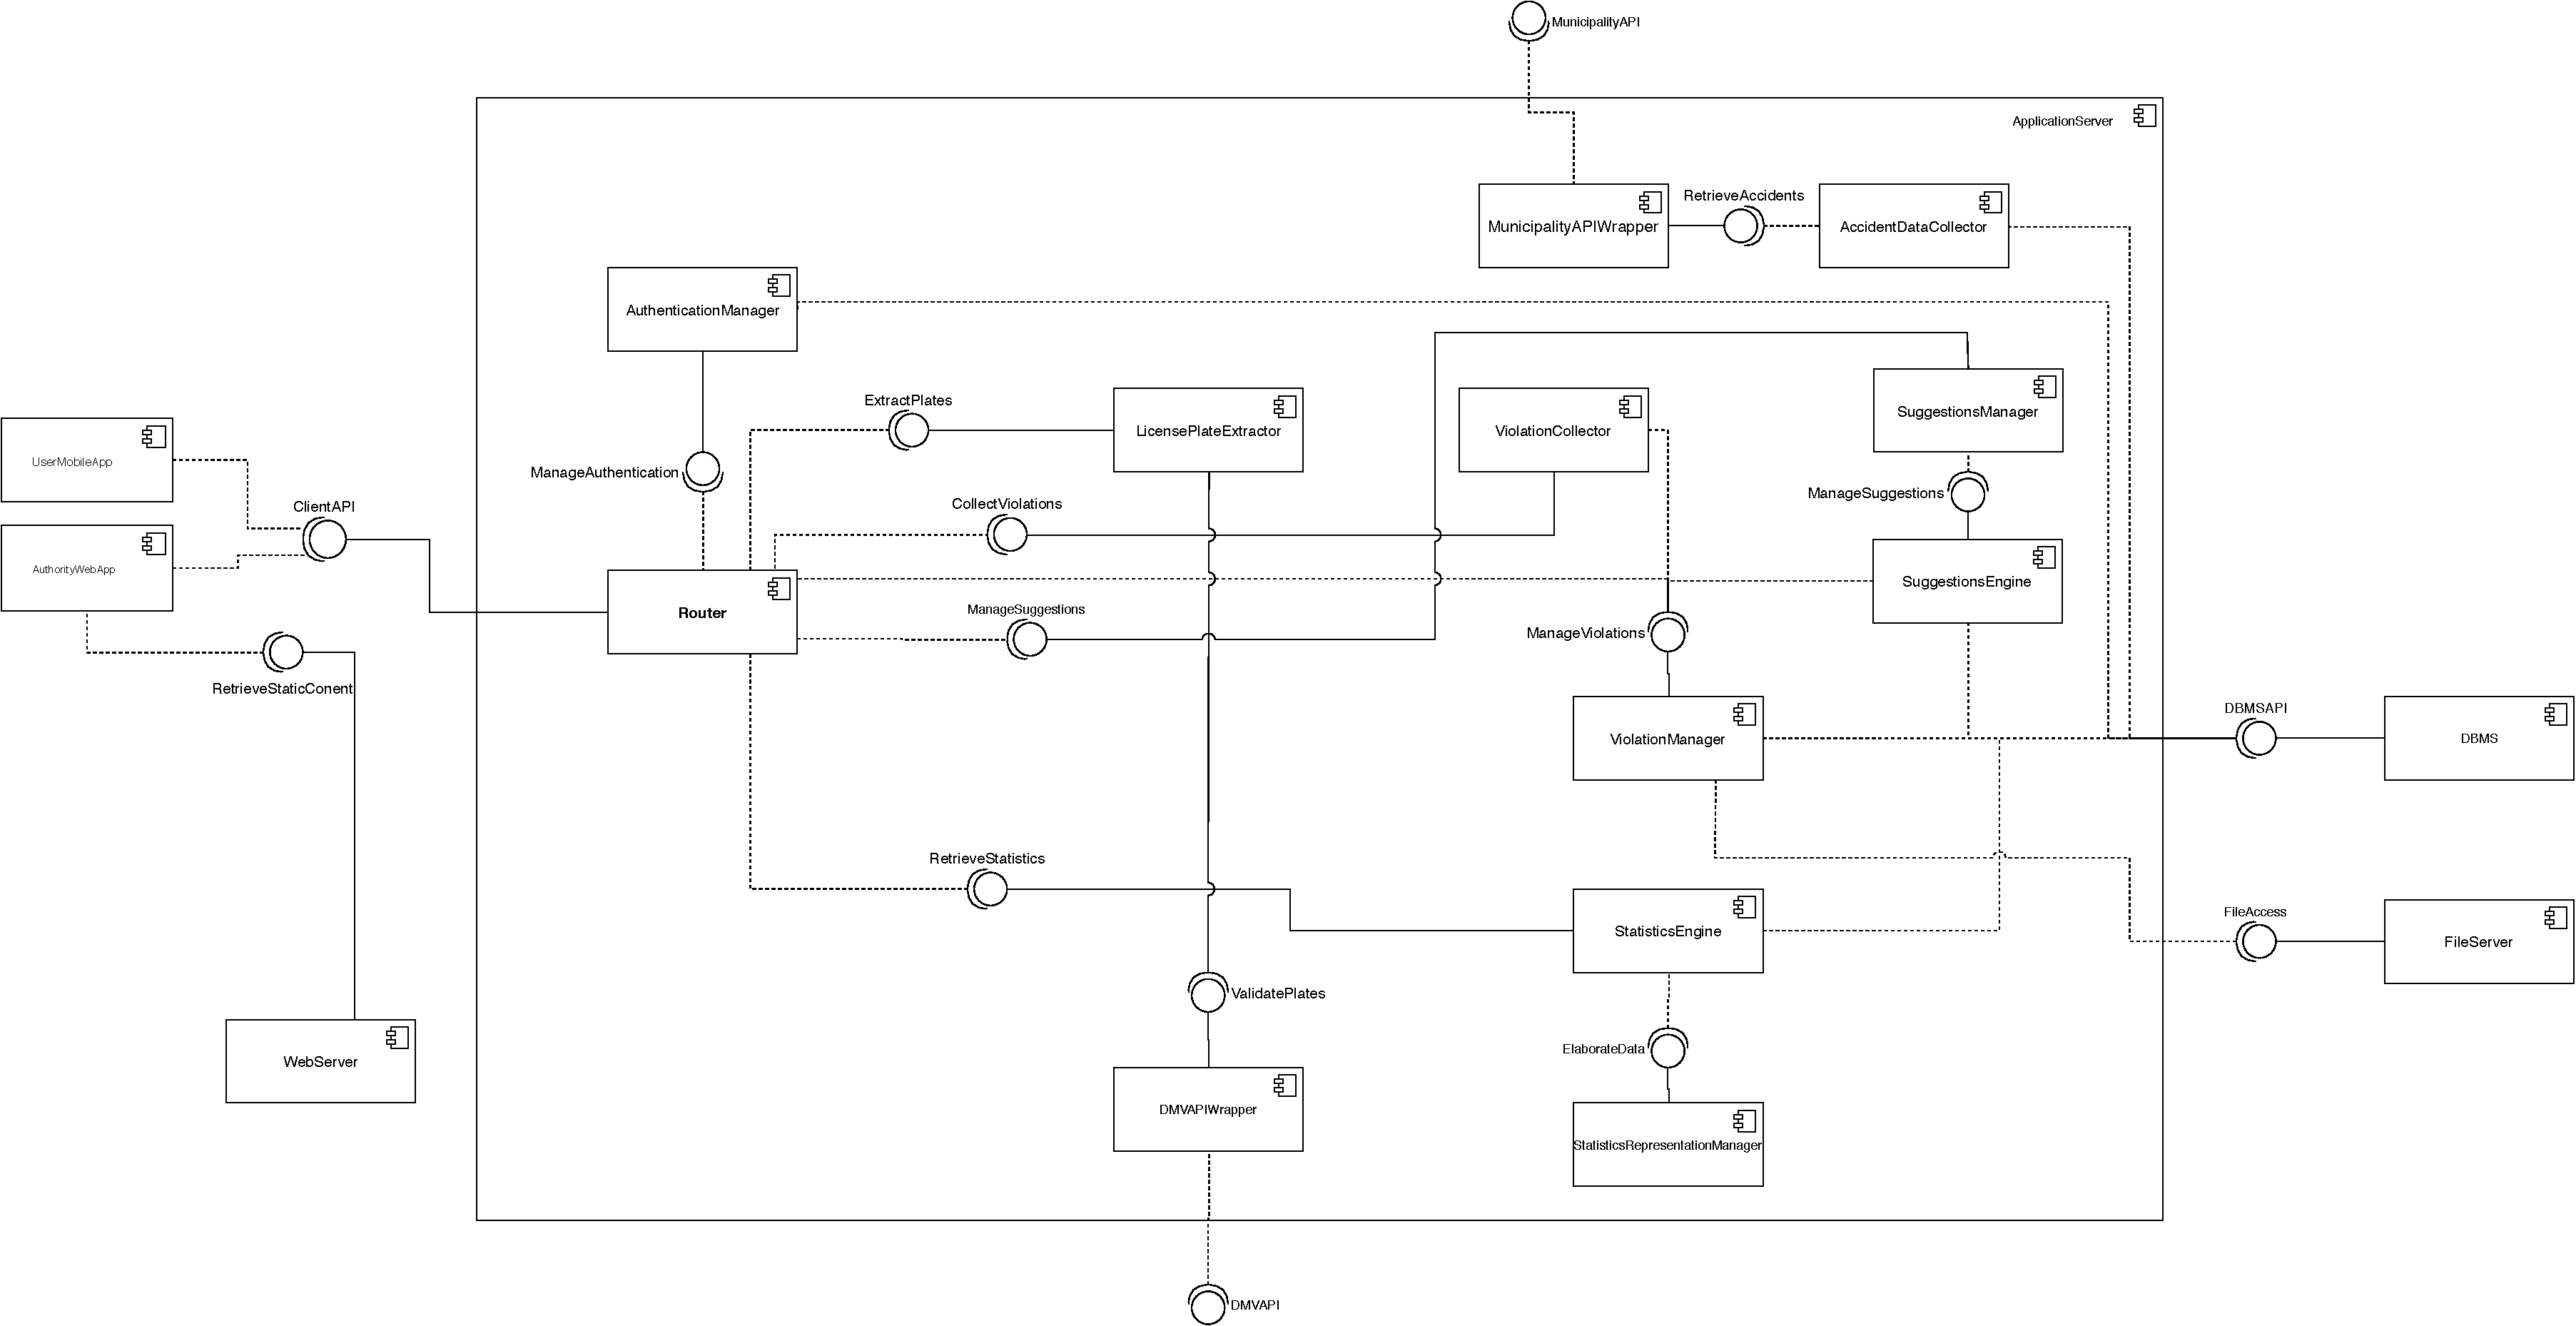
\includegraphics[width=\textwidth]{dd_component.pdf}
    \caption{Component Diagram, with an exploded view of the ApplicationServer
    subsystem.}
    \label{fig:component_diagram}
\end{figure}
\noindent
The system is composed of four subsystems:
\begin{description}
    \item[UserMobileApp] This is the smartphone app that provides all the
    functionalities to the citizens. It handles the presentation and the user
    interaction locally, while it interacts with the application server
    by using the \emph{ClientAPI} (RESTful).
    \item[AuthorityWebApp] This is the web application used by authorities.
    It handles the presentation and user interaction. The data to be displayed
    is retrieved using the REST API provided by the application server
    (\emph{ClientAPI}).
    \item[WebServer] This is a web server that provides static assets for the
    \emph{AuthorityWebApp}, such as HTML documents, the JavaScript code that
    runs the web app, CSS stylesheets and static images such as icons, etc.
    In this way web server replicas can be brought up or down depending on the
    current load. Since the replicas are all equal and completely stateless,
    each request can be equivalently routed to any of them.
    The only occasion in which the replicas must be synced is when a part of
    the web app code (or other asset) is changed, which can be considered a
    maintenance operation.
    \item[ApplicationServer] This is the component responsible for carrying
    out the business logic of the system. The application data related to
    SafeStreets is stored and retrieved from a relational DBMS.
    The component also accesses a file server to store and retrieve the images
    of the reported violations.
    Finally, it uses the interfaces offered by the Department of Motor Vehicles
    (\emph{DMVAPI}) and the various municipalities (\emph{MunicipalityAPI}).
    \item[DBMS] This component is the central relational database, used by the
    ApplicationServer. It stores all the application data that needs to be
    persisted (users, violations, retrieved accidents, municipality and
    authority info, access tokens), except the actual pictures of the
    violations. Of course, this component must not be implemented from scratch,
    but we just need to choose a commercially available solution that meets the
    requirements and configure it. It is required for the DBMS to support
    \emph{distribution} with a single transaction manager and also working with
    \emph{geographical data types}, to speed up queries based on locations.
    \item[FileServer] It is only responsible to store the images attached to
    the violation reports and making them available to be retrieved by the
    clients via the REST API.
\end{description}

\noindent
In figure \vref{fig:component_diagram} we further detail the internal components
of the \emph{ApplicationServer} subsystem, which is the core of the system.
Here we also provide a description of the various components and their
interactions:
\begin{description}
    \item[Router] This component exposes a public REST API, named
    \emph{ClientAPI} shared between the mobile and the web clients, which they
    use to perform all requests to the server (authentication and dynamic data
    in general). Each request type is assigned to a different REST endpoint
    (identified by an URL) and is then routed to the appropriate component,
    which will then carry it out autonomously and respond to the client
    (if required).
    \item[AuthenticationManager] It is responsible for the registration and
    login of both citizens and authority operators. Since it has to read and
    write user data, it needs to interact wit the \emph{DBMS}.
    This component is also responsible for handling sessions: after a successful
    login the component generates an \emph{access token} for the specific user,
    which is valid for a limited time. The token is then stored in the DB
    and can be accessed by the other components and finally it gets sent to the
    client that sent the login request.
    Now, when the client makes a request, it also provides the token which will
    be checked against the DB by the component that will handle the request.
    \item[LicencePlateExtractor] This component receives violation photos
    uploaded by the users and tries to extract the biggest licence plate
    number it an find in the photo. Then it checks if the detected plate exists
    by using the DMV API. If a valid licence plate number has been extracted,
    the component sends it to the client as a response, so it can autocomplete
    the licence plate field in the request report.
    This task has been separated from the violation reporting to take load
    off from the \emph{ViolationCollector} and also to give users the ability
    to manually insert the licence plate number if it couldn't be detected or
    to correct it.
    \item[ViolationManager] This component provides primitives to store,
    retrieve and review violations (i.e. mark them as accepted or discard them).
    It is used by the ViolationCollector to store an incoming violation and in
    this regard it is responsible to check and assign it to a responsible
    authority, based on the municipality in which the violation occurred. If
    this fails, the violation cannot be stored. Storing the violation also
    includes saving its attached photo to the \emph{FileServer}.
    In turn, when an operator requests to review violations, this components is
    activated and it is responsible to only retrieve the violations assigned to
    the requesting authority and sending them as a response.
    When the operator decides to mark a violation as accepted or discarded, this
    component is responsible for applying the change in the DB; note that it is
    necessary to check that the violation was assigned to the requesting
    authority by using the access token provided with the request.
    \item[ViolationCollector] This component is responsible to handle incoming
    violation reports from the users, in particular to check their validity and
    then use the \emph{ViolationManager} to store them in the DB.
    In particular, it checks that the report contains all the required fields
    and that the licence plate number is valid (by using the DMV API).
    \item[StatisticsEngine] This component is responsible for computing
    statistics for both users and authorities. A statistics request will come
    in, indicating the type of statistics (e.g.\ violations per month) and
    possibly various filters (e.g.\ municipality, year, \dots); the component
    will perform a query to the DB and compute the required statistics.
    These are then passed on to the \emph{StatisticsRepresentationManager}
    and the result is sent as a response to the client.
    \item[StatisticsRepresentationManager] Given some \emph{raw} statistics,
    this component is responsible to generate their appropriate representation
    to be fed to the client libraries used to show statistics.
    This takes into account the diagram colors, text labels, measurement units
    and all the parameters needed by the client libraries to visualize the
    appropriate diagram.
    The reason for this to be done server-side is that we don't have to send
    raw data over the network and we can provide a consistent representation
    between the mobile app and the website (in terms of colors, labels, etc.).
    \item[AccidentDataCollector] This component is responsible for periodically
    collecting data about accidents from the municipalities that provide it
    and store it to the database. As we stated in the RASD, we assume that the
    municipalities provide an API to retrieve all accidents that have been
    registered after a certain date; the component can rely on this to perform
    incremental updates, rather than retrieving all the data each time.
    Since the accident data will be used to compute suggestions, a task that
    requires a lot of accesses, we chose to store it locally rather than
    continuously contacting the municipality API. This is also dictated by
    the fact that we have no control over the availability of the external
    data sources.
    \item[SuggestionsEngine] This component is responsible to periodically
    compute new suggestions for the authorities that have activated the
    \emph{SmartSuggestions} functionality.
    It reads data about violations and accidents directly from the DB and
    then computes the suggestions by using Machine Learning algorithms.
    These suggestions are then stored into the DB, so they can be retrieved
    by the authority. Note, however, that no notification is actively sent to
    the authority.
    Furthermore, since there can be a lot of municipalities involved, the
    component should also be able to schedule its jobs over time, in order to
    keep up to date with new violations and accidents data.
    \item[SuggestionsManager] Provides methods to retrieve suggestions and
    mark them as carried out. Analogously to \emph{ViolationManager} it receives
    requests by authority web apps containing an access token, and it has to
    allow access only to the suggestions for the authority that owns the token.
    \item[DMVAPIWrapper] The components that need to check the validity of
    a licence plate number don't directly interact with the external API, but
    with this internal component that wraps around the API.
    Its aim is to provide an interface that is consistent with the rest of the
    internal ones. This makes it easier to hide the actual API and data format
    used by the external service, so if it changes for some reason we only
    need to modify this component rather than all the ones that rely on this
    service.
    \item[MunicipalityAPIWrapper] Similarly to the previous one, we provide a
    wrapper also for the APIs offered by municipalities to retrieve data about
    accidents. Here the need for a component that converts the various data
    formats provided by the external APIs to an internal, shared format is
    even more evident, since it is quite unlikely that all the municipalities
    provide such data in the same format.
\end{description}\clearpage
\section{Deployment view}
\label{sec:deployment_view}
\begin{figure}[ht]
    \centering
    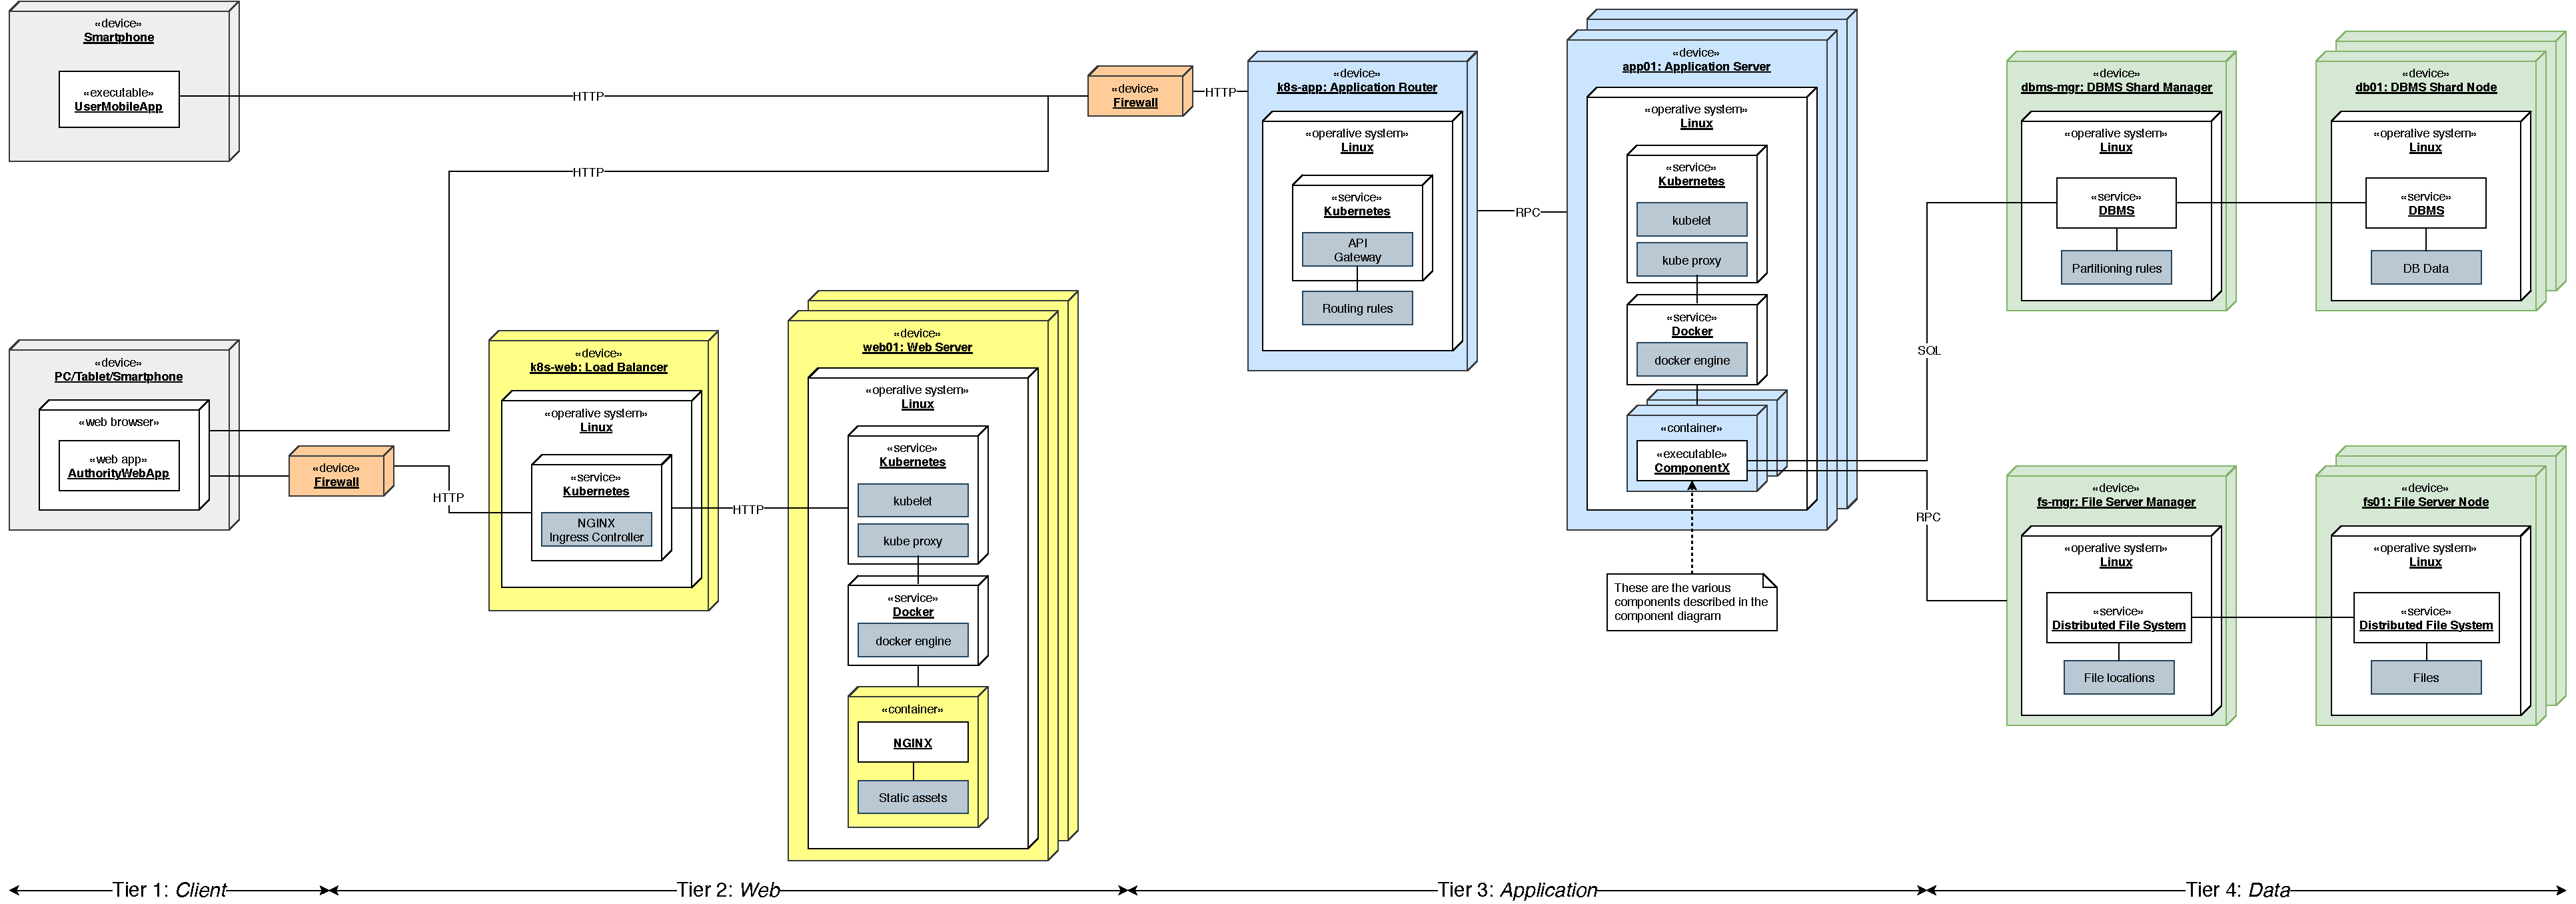
\includegraphics[width=\textwidth]{dd_deployment}
    \caption{Deployment diagram}
    \label{fig:depolyment_diagram}
\end{figure}

The diagram in figure~\vref{fig:depolyment_diagram} shows the deployment plan
for the various components of the system. External components (such and the DMV
and municipality systems) are not shown, since they are already built and
deployed, and they can just be accessed from the internet.
The diagram shows the \emph{physical devices} in which the components will run,
the \emph{communication channels} between the components and their
\emph{software environment}.
The system is split into \emph{four tiers}, the last three heavily relying on
replication to achieve scalability and fault tolerance. It is worth pointing out
that tier 1 and 4 correspond to the \emph{presentation} and \emph{data} layers
identified in section~\ref{sec:overview}, while the \emph{application} layer
has been separated in tiers 2 and 3.

\begin{description}
    \item[Client tier] It is composed by the end-user interfaces:
    the \emph{mobile application} for the citizen and the \emph{web application}
    for the authority.
    The first one must be developed for both Android and iOS, as required in
    the RASD, and communicates directly to the application tier by using
    HTTP (specifically a REST API).

    The website, on the other hand, only requires a web browser to be used,
    and therefore it can run on PCs, as well as tablets and smartphones,
    although the focus should be mainly on PCs.
    It interacts with the web tier through HTTP (to request static assets)
    and to the application tier also through HTTP, using the REST API.
    \item[Web tier] This tier contains the \emph{WebServer} component,
    represented by NGINX, which has been chosen for its reliability and
    performance for static serving.
    NGINX actually runs inside a Docker container, which also contains the HTML,
    CSS and JS files to be served. The containers are orchestrated by
    \emph{Kubernetes}, which takes care of auto-scaling, load balancing, image
    and configuration deployment thanks to the \emph{NGINX Ingress Controller}.
    There is a single node (\emph{k8s-web}) that acts as a Kubernetes manager.
    It is worth pointing out that, since NGINX already uses internal workers,
    there are no advantages on deploying more than one container to each
    replicated node.
    \item[Application tier] This tier is responsible for the components that
    implement the business logic of the system, see section~%
    \ref{sec:component_view} for more details on them.
    As in tier 2, we rely on Kubernetes and Docker for replication.
    Here the Kubernetes manager (\emph{k8s-app}) implements the \emph{Router}
    component through an API gateway module.
    The role of this module is to accept REST requests and route them to
    the correct container as remote procedure calls (RPCs).
    Each container runs a specific application component and they communicate
    between themselves through RPC. Differently from tier 2, here it makes sense
    to run multiple containers on the same node.
    \item[Data tier] This tier contains the components responsible for
    persistently storing data: the database and the file server.
    The database component is implemented as a Relational Database Management
    System (RDBMS), to which application components send SQL queries.
    Since the data stored in the DB will most likely exceed the capacity of a
    single node over time, it is horizontally partitioned over multiple nodes
    using \emph{database sharding} (see section~\ref{subsec:db_sharding}):
    there is a single node that acts as the transaction manager, while the
    actual data resides on the \emph{shard nodes}.

    The consideration made for the DB also holds for the file server: at one
    point the collected images will exceed the capacity of a single node.
    In the same way the files are partitioned over multiple nodes and there is
    a single manager that keeps the mapping between the file names and their
    actual locations. The communication with the application tier relies on RPC.
    
    In this way the application tier only sees one entrypoint for the DBMS and
    one for the file server, which hide the internal replication.
\end{description}

\noindent
For more details on the design choices, in particular how data is partitioned
between nodes (and also under which assumptions),
see section~\ref{sec:styles_patterns}.
\clearpage
\section{Runtime View}
In this section all the basic interactions will be described. All the use cases
from the RASD document are visualized in a deeper way. The Application Server is
exploded in the various components, just like in Figure
\ref{fig:component_diagram}, and also the interaction between the components is
described.

\begin{figure}[h]
    \centering
    \includegraphics[width=\textwidth]{dd_sequence_diagram_uc_1_1}
    \caption{Registration process for a new User}
    \label{fig:dd_sequence_diagram_uc_1_1}
\end{figure}

\begin{figure}[h]
    \centering
    \includegraphics[width=\textwidth]{dd_sequence_diagram_uc_1_2}
    \caption{Login process for a User}
    \label{fig:dd_sequence_diagram_uc_1_2}
\end{figure}

\begin{figure}[h]
    \centering
    \includegraphics[width=\textwidth]{dd_sequence_diagram_uc_1_3}
    \caption{Violation Report process for a User}
    \label{fig:dd_sequence_diagram_uc_1_3}
\end{figure}

\begin{figure}[ht]
    \centering
    \includegraphics[width=\textwidth]{dd_sequence_diagram_uc_1_4}
    \caption{Visualize Statistics process for a User}
    \label{fig:dd_sequence_diagram_uc_1_4}
\end{figure}

Note that Figure \ref{fig:dd_sequence_diagram_uc_1_4} shows the interaction
between Safe Streets and the User but the same action can be done by the
Authority Operator as well. In the latter case, there are no substantial
differences from the former case, so another dedicated Sequence Diagram is not
necessary.

\begin{figure}[h]
    \centering
    \includegraphics[width=\textwidth]{dd_sequence_diagram_uc_2_1}
    \caption{Violation management process for the Authority}
    \label{fig:dd_sequence_diagram_uc_2_1}
\end{figure}

\begin{figure}[h]
    \centering
    \includegraphics[width=\textwidth]{dd_sequence_diagram_uc_2_3}
    \caption{SmartSuggestions management for the Authority}
    \label{fig:dd_sequence_diagram_uc_2_3}
\end{figure}

\begin{figure}[ht]
    \centering
    \includegraphics[width=\textwidth]{dd_sequence_diagram_accident_collector}
    \caption{Periodic routines to fetch and process accident data}
    \label{fig:dd_sequence_diagram_accident_collector}
\end{figure}

Lastly, in Figure \ref{fig:dd_sequence_diagram_accident_collector}, we can see
how accident data is fetched from the Municipality API, and then how it is
processed from the SuggestionsEngine component. It is important to underline
that no notification will be pushed to the Authority Web App when new
Suggestions are available, they will be shown to the Operator once he selects
the \emph{SmartSuggestions} page.

\clearpage
\section{Component Interfaces}
In Figure \ref{fig:interface_diagram} all the various interfaces are shown. The
interface \emph{Client API} is divided into two separate sub-interfaces in order
to clarify the two main functions of the Router component: it has to handle both
the User Mobile App and the Authority Web App. An exploded view of the
\emph{Client API} interface is shown here in Figure \ref{fig:router_interface}.
A detailed explanation of the use of the various methods provided by the
interfaces is not necessary since those exact names are used in the Sequence
Diagrams, furthermore the names are mostly self-explanatory.

\begin{figure}[h]
    \centering
    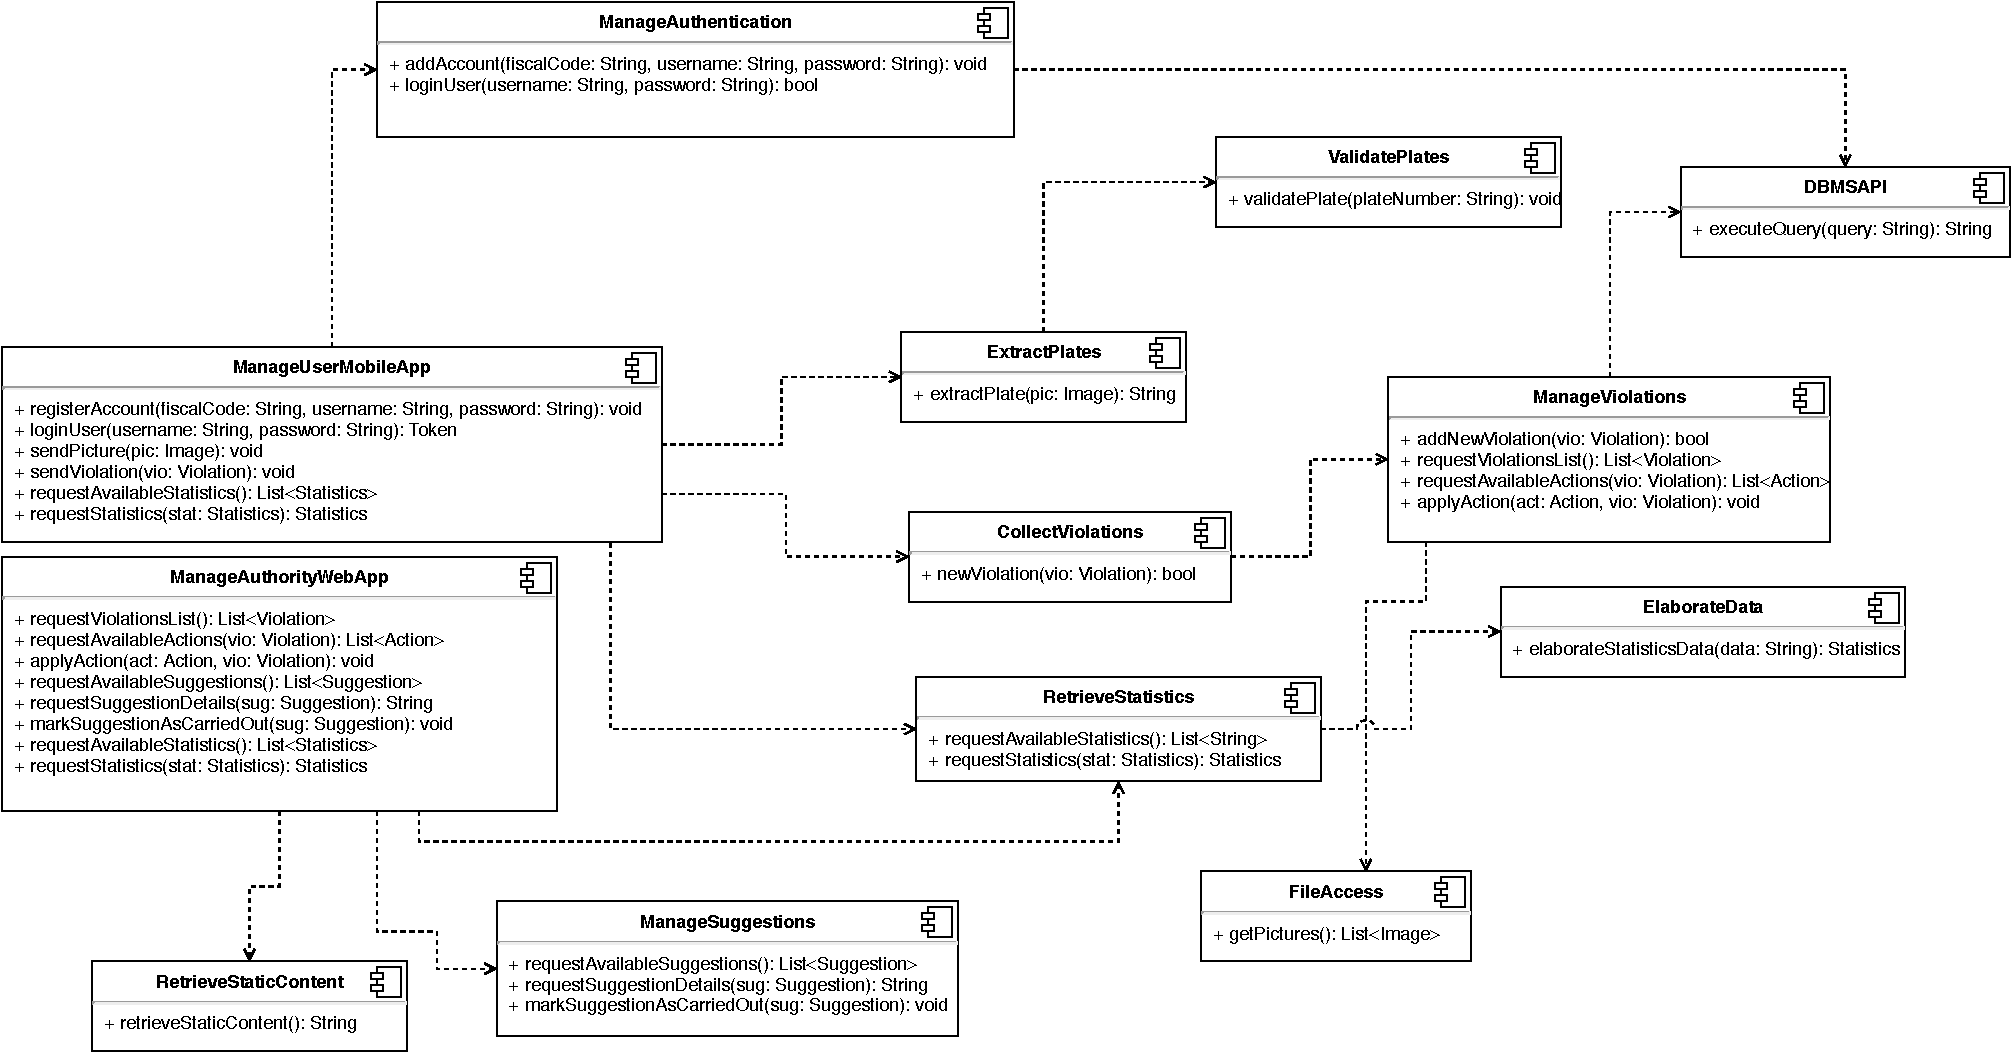
\includegraphics[width=\textwidth]{interface_diagram.pdf}
    \caption{Interfaces that are used in the Application Server}
    \label{fig:interface_diagram}
\end{figure}

\begin{figure}[h]
    \centering
    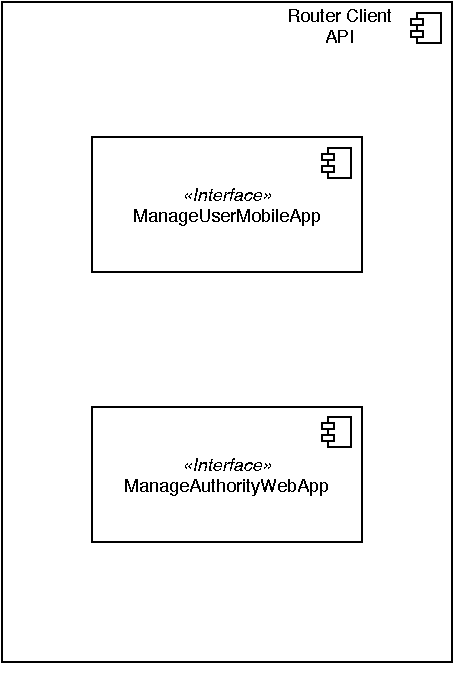
\includegraphics[width=5cm]{router_interface.pdf}
    \caption{Exploded view of the interface provided by the Router component}
    \label{fig:router_interface}
\end{figure}\clearpage
\section{Selected architectural styles and patterns}
\label{sec:styles_patterns}
\subsection{Four-tier client/server architecture}
As shown in section~\ref{sec:deployment_view}, we decided to use a client/server
architecture, where the components have been divided into four \emph{tiers}.
The communication is always initiated by the client, while the server only
waits for requests, processes them and finally responds. There are no cases
in which the server actively contacts the client (e.g.\ push notifications).
The client/server communication is fully based on HTTP.
Furthermore, in order to guarantee security, it is mandatory to use HTTP over
TLS (HTTPS) for such communication.

On the other hand the division in tiers enables to \emph{uncouple} the
components from one another, which facilitates parallel development, maintenance
and also hides the internal complexity of a tier (e.g.\ partitioning and
replication) to its users.

\subsection{RESTful communication and stateless components}
As already mentioned earlier, the communication between the client and the
application tier is based on the REST architectural style. Here both the mobile
and the web clients can perform operations (register, login, mark violations and
suggestions) and request data (violations, suggestions, statistics) in a
request-response fashion. In fact all the above mentioned functionalities are
designed in such a way that they can each be completed with a single request and
response. Furthermore each request also carries an access token (except
registration and login, of course) that is used to check the access rights of
the client who sent the request.
In this way the application components can be \emph{completely stateless} and
only rely on the data stored in the DB and file server.
This means that we can have multiple instances of the same component and the
\emph{Router}, implemented with a Kubernetes API Gateway, can forward an
incoming request to any of those instances.

Another advantage of using the RESTful architecture is that data can be
represented in a simple and platform-independent way using JSON, allowing for
a total uncoupling between the application server and the clients.
In fact, even if the citizen client is a native iOS or Android application,
while the authority client is a website, they can still share the same API,
as the conversion to the concrete data structures happens inside the client
itself.

\subsection{Elastic components and load balancers}
The choice of a RESTful architecture with stateless components means that a
request can be sent to any instance of a component, without affecting the
correctness of the response. These considerations of course hold also for
the static web server, which is stateless by definition.

We have exploited this advantage by running each component in a separate
\emph{Docker} container and all containers are managed by Kubernetes.
Kubernetes always keeps at least one instance of each component running, but
when the workload increases it automatically spawns new containers to replicate
stressed components and automatically assigns the requests to the various
instances in order to share the workload between them.
When the workload decreases again, the replicated containers are deleted
accordingly.

The goals of this decision are to achieve \emph{scalability} and also to make
an efficient use of the computational resources.

\subsection{Facade pattern}
The facade pattern consist in providing a unique and simplified interface to
interact with a complex system. This pattern has been used various times
in our design:
\begin{itemize}
    \item in the \emph{ApplicationServer} subsystem, which provides a unique
    REST API managed by the \emph{Router}. This hides the fact that the requests
    are actually fulfilled by other components, which may also be replicated
    other multiple nodes.
    \item in the \emph{data tier}, where both the Database and the File Server
    offer a single entrypoint to access data that is actually partitioned over
    multiple nodes.
\end{itemize}

\subsection{Adapter pattern}
\label{subsec:adapter_pattern}
This pattern consists in allowing an existing interface to be used as another
interface. We used this pattern on the \emph{DMVAPIWrapper} and
\emph{MunicipalityAPIWrapper}, both providing access to external APIs.
The external APIs are usually not consistent with the internal ones, in
terms of communication model (RPC in this case), data format (the data
structures may be different) and they may also change over time.
So the aim of the above mentioned components is to provide interfaces that are
consistent with the rest of the internal ones. If an external API changes for
some reason we only need to modify its wrapper, rather than all the components
that use it.

\subsection{Database sharding}
\label{subsec:db_sharding}
Database sharding is a database architecture pattern that consists in
\emph{horizontal partitioning}: separating the table rows into different
sub-tables (\emph{logical shards}) and assigning each of them to
a different node (\emph{physical shard})~\cite{digitalocean:db-sharding}.

This choice has been dictated by the fact that we expect that, at some point,
a single DB node wouldn't be able to store all the data, so we needed to apply
a \emph{horizontal scaling} technique that allows to efficiently partition the
data and share the workload between different nodes.

In order to actually balance the workload between the physical shards, a proper
partitioning criterion should be put in place.
We chose to create \emph{a logical shard for each authority}, meaning that
all the violations and suggestions regarding the municipalities under a specific
authority belong to the same shard. The rationales that led to this choice are:
\begin{itemize}
    \item a single authority has access to all and only the data about the
    municipalities under its jurisdiction
    \item the suggestions are computed on a per-municipality basis, so they
    only access data about a specific municipality
    \item the rate of requests for a single municipality (or a small subset)
    is relatively small and can be supported by a single node
    \item the rate of requests is (approximately) evenly spread between
    the municipalities
\end{itemize}
With this technique, the most common operations (retrieve suggestions and
violations, insert or update a single violation or suggestion) only require
access to a single partition, which makes them efficient.

  \chapter{User interface design} \label{ch:ui}
\label{ch:ui_design}
As already stated earlier, we have different interfaces for the mobile
application and the web application.
The main idea is to initially establish a common design language (colors,
fonts, look of reusable components) which can then be applied to both
interfaces. In this regard we have provided some early mockups of the main pages
of both interfaces in the RASD (subsection 3.1.1 -- User interfaces).

Here we give a better detail of the flow of the application, also including
some pages of minor importance that were not shown in the RASD.
In the following diagrams the boxes represent the different pages and the
arrows the transitions from a page to another. The arrow labels indicate the
conditions(s) which trigger a particular transition.

\begin{figure}[ht]
    \centering
    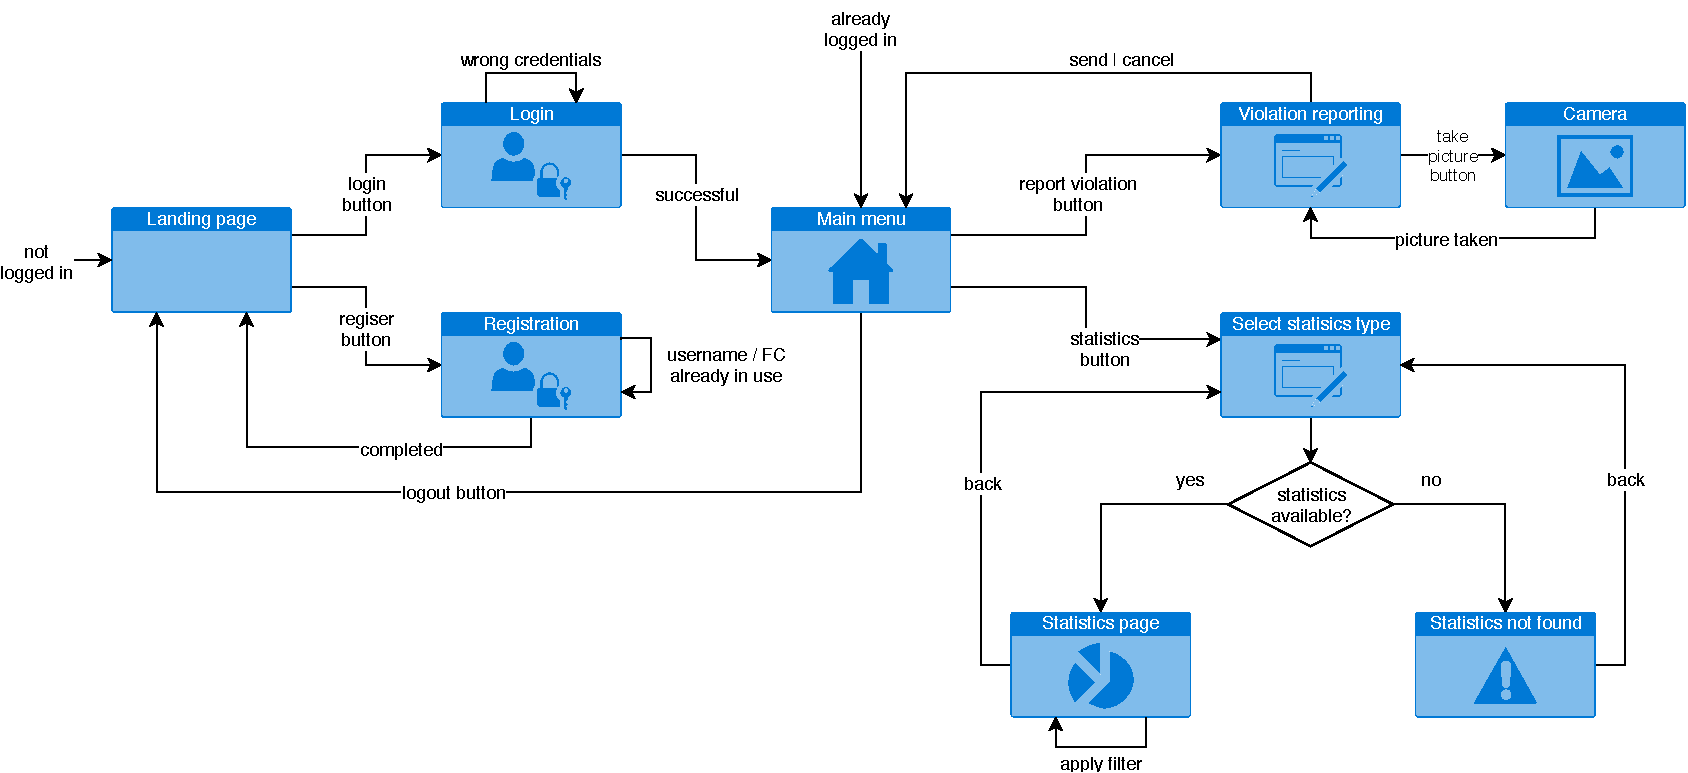
\includegraphics[width=\textwidth]{dd_ux_mobile}
    \caption{UX diagram for the mobile app}
    \label{fig:ux_mobile}
\end{figure}

Figure \vref{fig:ux_mobile} shows the UX diagram for the mobile application.
When the user opens the application on his smartphone, the first check is
whether he is already logged in or not. If he's not, the \emph{landing page}
will be shown, which enables him to login or register, otherwise the user
is directly taken to the \emph{main menu}.
Once in the \emph{main menu} the user can decide whether to report a violation,
view statistics or log out (this was not shown in the previous mockups).
For conciseness the links to come back from this page are not shown in the
diagram.

In case the user decides to report a violation, he will be taken to the
\emph{violation reporting page}, which is essentially a form that also
requires to take a photo. The process of reporting a violation has been already
described in the use cases.

In case the user decides to view statistics, he will be first presented
with a set of possible types of statistics (e.g.\ by month, by type).
He will select one of these types and the system will try to compute those
statistics. In case they are not available (e.g.\ there is no sufficient data
for violations in the surrounding area), then the user is brought to an
\emph{error page} from which he can go back and try with another type.
If everything goes right, instead, the user is brought to the
\emph{statistics page}; note that here the rendering of the statistics
(histogram, map, list) depends on the selected type. From here the user
can apply additional filters (restrict to a specific area, time period
or violation type).

\begin{figure}[ht]
    \centering
    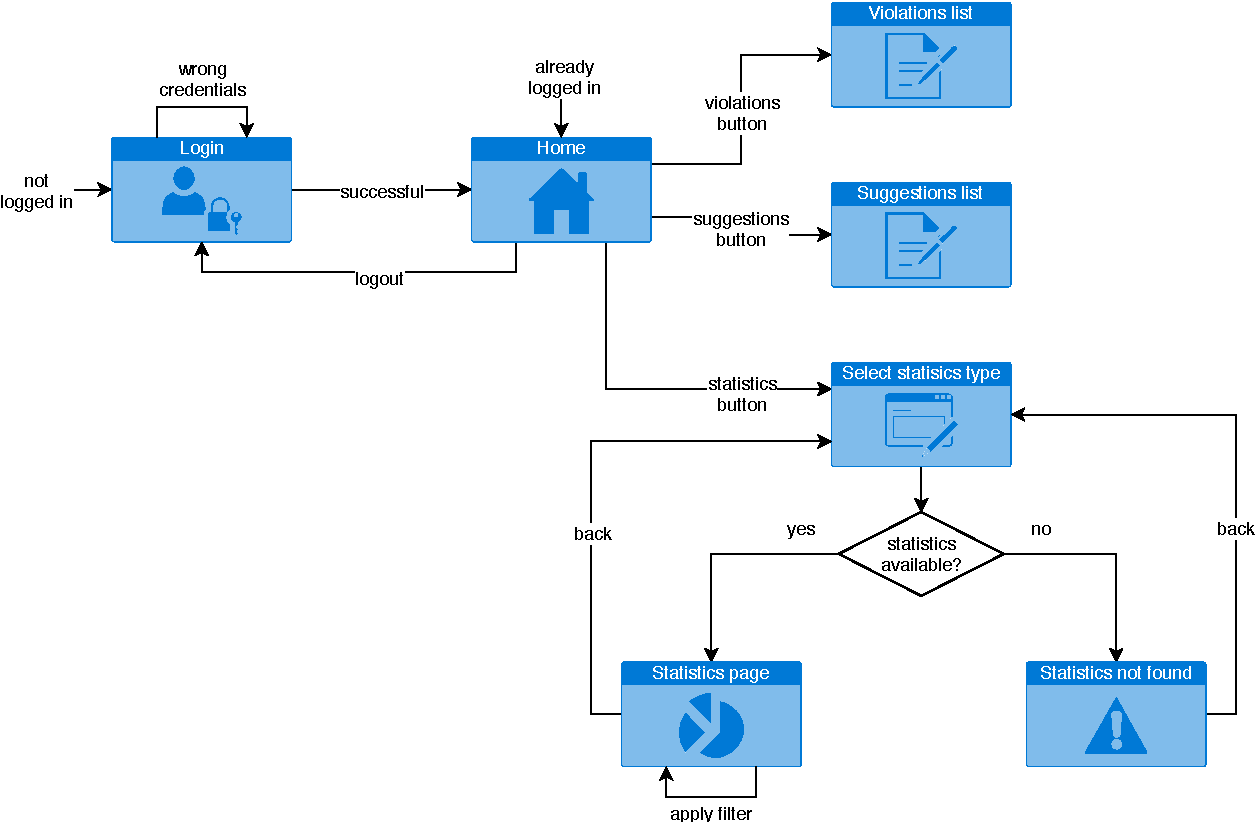
\includegraphics[width=\textwidth]{dd_ux_web}
    \caption{UX diagram for the web app}
    \label{fig:ux_web}
\end{figure}

Figure \vref{fig:ux_web} shows the UX diagram for the web application.
When the operator navigates to the website he will be presented with a
\emph{login page} if he's not already logged in, otherwise he will be
taken directly to the \emph{main menu}.
From the \emph{main menu} the operator can access the main functionalities
of the system, and he can also decide to \emph{log out}.

In case he clicks on the violations button, he will be taken to the
\emph{violations list} page, which shows all the most recently reported
violations that belong to that specific authority; violations that are still
pending for approval are shown at the top.
From here the operator can click on the \emph{info button} of a violation:
this will expand the list item to a card that shows the details of a the report.
If the violation is still unrevised, this card will also contain an two action
buttons to accept or discard the violation, respectively.
The list of violations can be implemented as an \emph{infinite scrolling list}:
initially only the most recent $N$ violations are retrieved, enough to fill
the page; then as the operator scrolls down the next $N$ violations are
retrieved from the server, and so on.

The suggestions button is only shown if the \emph{SmartSuggestions}
functionality is active for the current municipality. If the operator clicks on
it he's taken to the \emph{suggestions list} page.
This is very similar to the previous one, because it involves viewing a list
of suggestions, some of which are new and can be expanded to be marked as
\emph{carried out}. Also here we can apply the technique of the
\emph{infinite scrolling list}.

If the operator clicks on the statistics button, the process is pretty much the
same of the mobile application, detailed before.
The only things to keep in mind are that the authority also has the possibility
to see the licence plate numbers associated to violations.
Here, since this page will primarily viewed on the large screen of a PC,
we can show more data in a single page than in the mobile application
(as suggested by the mockups).

As an additional consideration, since the website can be viewed from devices
(smartphone, tablets, laptops, desktop PCs), its interface can be made
\emph{responsive} to adapt to the various screen sizes. At least this should be
done for the \emph{violations list} page, which can be useful for field
operators.
  \chapter{Requirements traceability} \label{ch:req}
\label{ch:req_traceability}
The system design described in this document must meet the requirements --
both functional and non-functional -- defined in the RASD. We dedicate this
chapter to mapping each requirement to the various elements we designed to
fulfill it.

\section{Functional requirements}
The functional requirements are mainly related to \emph{components}, so for each
requirement we list the related components and a brief explanation when needed,
for a detailed description of each component's purpose see
section~\ref{sec:component_view}. Please note that for conciseness we only list
the components that are \emph{directly related} to satisfy the requirement,
other components, such as the DB, that are indirectly used might be omitted.

\begin{description}
    \RuleItem{R1} % user registration
    \begin{itemize}
        \item \emph{UserMobileApp} -- interface provided to the user
        \item \emph{AuthenticationManager} -- creates the accounts, enables
        login
    \end{itemize}

    \RuleItem{R2} % check registration data
    \begin{itemize}
        \item \emph{AuthenticationManager} -- checks unique username and
        password before creating an account
    \end{itemize}

    \RuleItem{R3} % upload photos
    \begin{itemize}
        \item \emph{UserMobileApp} -- contains page to take photo
        \item \emph{LicencePlateExtractor} -- accepts photos uploaded by users
        to extract the licence plate
        \item \emph{ViolationCollector} -- accepts photos attached to incoming
        violation reports
    \end{itemize}

    \RuleItem{R4} % auto-detect report fields
    \begin{itemize}
        \item \emph{UserMobileApp}
    \end{itemize}

    \RuleItem{R5} % select violation type
    \begin{itemize}
        \item \emph{UserMobileApp} -- report violation page
        \item also enforced by the DBMS schema
    \end{itemize}

    \RuleItem{R6} % send reports
    \begin{itemize}
        \item \emph{UserMobileApp} -- report violation page
        \item \emph{ViolationCollector} -- accepts incoming violation reports
    \end{itemize}

    \RuleItem{R7} % edit report before sending
    \begin{itemize}
        \item \emph{UserMobileApp} -- report violation page
    \end{itemize}

    \RuleItem{R8} % detect invalid licence plates
    \begin{itemize}
        \item \emph{DMVAPIWrapper}
    \end{itemize}

    \RuleItem{R9} % extract licence plate
    \begin{itemize}
        \item \emph{LicencePlateExtractor}
    \end{itemize}

    \RuleItem{R10} % persistent storage
    \begin{itemize}
        \item \emph{DBMS} -- persistently stores the data about the reports,
        except for the image files
        \item \emph{FileServer} -- persistently stores the photos attached to
        the violation reports.
    \end{itemize}

    \RuleItem{R11} % only persist valid violations
    \begin{itemize}
        \item \emph{ViolationCollector} -- checks the validity of the fields
        in the incoming reports
        \item  \emph{ViolationManager} -- assigns each incoming report to an
        authority, if this is not possible the report is rejected, otherwise it
        is sent to the DBMS
        \item \emph{DBMS} -- enforces integrity constraints on the fields of the
        stored violation reports
    \end{itemize}

    \RuleItem{R12} % save anonymous reports
    \begin{itemize}
        \item \emph{DBMS} -- in the schema a violation is not related to a user
        (also see~\ref{fig:er_diagram})
    \end{itemize}

    \RuleItem{R13} % operator login
    \begin{itemize}
        \item \emph{AuthorityWebApp} -- interface for the operator, also saves
        the access token returned by the server
        \item \emph{AuthenticationManager} -- checks login credentials and
        creates and returns an access token
        \item \emph{DBMS} -- stores the login credentials
    \end{itemize}

    \RuleItem{R14} % assign violation to authority
    \begin{itemize}
        \item \emph{UserMobileApp} -- captures the location of the user and
        sends it as part of the report
        \item \emph{ViolationManager} -- assigns each incoming report to an
        authority, if this is not possible the report is rejected
        \item \emph{DBMS} -- stores the municipalities for which an authority
        is responsible
    \end{itemize}

    \RuleItem{R15} % operator only accesses violations under jurisdiction
    \begin{itemize}
        \item \emph{AuthorityWebApp} -- violations list page
        \item \emph{ViolationManager}
    \end{itemize}

    \RuleItem{R16} % delete discarded reports
    \begin{itemize}
        \item \emph{AuthorityWebApp} -- violations list page
        \item \emph{ViolationManager}
    \end{itemize}

    \RuleItem{R17} % filter and aggregate violations
    \begin{itemize}
        \item \emph{DBMS} -- SQL provides the \texttt{where} and \texttt{group
        by} clauses in its query language
    \end{itemize}

    \RuleItem{R18} % compute statistics
    \begin{itemize}
        \item \emph{StatisticsEngine}
    \end{itemize}

    \RuleItem{R19} % view violations (operator)
    \begin{itemize}
        \item \emph{AuthorityWebApp} -- statistics page
        \item \emph{StatisticsEngine} -- computes statistics, includes the plate
        number based on the access token in the request
        \item \emph{StatisticsRepresentationManager} -- formats the raw
        statistics data
    \end{itemize}

    \RuleItem{R20} % view violations (user)
    \begin{itemize}
        \item \emph{UserMobileApp} -- statistics page
        \item \emph{StatisticsEngine} -- computes statistics, includes the plate
        number based on the access token in the request
        \item \emph{StatisticsRepresentationManager} -- formats the raw
        statistics data
    \end{itemize}

    \RuleItem{R21} % retrieve accident data
    \begin{itemize}
        \item \emph{MunicipalityAPIWrapper}
        \item \emph{AccidentDataCollector}
    \end{itemize}

    \RuleItem{R22} % determine causal relation between accidents and violations
    \begin{itemize}
        \item \emph{SuggestionsEngine}
    \end{itemize}

    \RuleItem{R23} % determine suggested actions
    \begin{itemize}
        \item \emph{SuggestionsEngine}
    \end{itemize}

    \RuleItem{R24} % view and manage suggestions
    \begin{itemize}
        \item \emph{AuthorityWebApp} -- suggestions list page
        \item \emph{SuggestionsManager} -- get list of suggestions, mark them
    \end{itemize}

    \RuleItem{R25} % feedback
    \begin{itemize}
        \item \emph{SuggestionsEngine}
    \end{itemize}
\end{description}
\section{Non-functional requirements}
The non-functional requirements, which comprise the \emph{performance
requirements}, \emph{design constraints} and \emph{software system attributes}
(sections 3.3-3.5 of the RASD), are particularly related to the \emph{deployment
strategy} (see section~\ref{sec:deployment_view}) and the \emph{architectural patterns}
(see section~\ref{sec:styles_patterns}) that have been applied.
Here we analyze in how the crucial aspects have been taken care of.

\paragraph{Scalability}
A lot of architectural decisions have been made to ensure the scalability of
the system:
\begin{itemize}[noitemsep]
    \item tiered architecture
    \item containerization of components with Docker and Kubernetes
    \item elastic replication and load balancing
    \item stateless components
    \item database sharding
\end{itemize}
These are also aimed at improving the \emph{reliability}, \emph{availability}
and reduce \emph{response times}.

\paragraph{Performance}
Aside from the response times for the clients, it has been required for the
suggestions to be generated periodically. As stated in
section~\ref{sec:component_view} the \emph{SuggestionsEngine} will take care of
scheduling the jobs to generate new suggestions, as new data becomes available.

\paragraph{Security}
The measures related to security include:
\begin{itemize}[noitemsep]
    \item firewalls to protect the internal components
    (section~\ref{sec:deployment_view})
    \item use of HTTPS for communication over the internet
    (section~\ref{sec:deployment_view})
    \item hashed passwords in the DB
    (sequence diagram~\ref{fig:dd_sequence_diagram_uc_1_1})
    \item session tokens to use the APIs (section~\ref{sec:component_view})
\end{itemize}

\paragraph{Mantainability}
The use of the RESTful architecture (section~\ref{sec:styles_patterns}) and the
loose coupling between the components are all aimed at providing a better
maintainability than a monolithic approach.
Furthermore the use of management tools such as Kubernetes provide a way of
managing and distributing images of the various components, which facilitates
the versioning and deployment processes.

\paragraph{Portability}
The \emph{mobile application} will be developed for both Android and iOS
platforms, keeping a consistent design language and user experience.
On the server side, the use of \emph{containerization} reduces the dependency
of the components from the hardware, since they run on a virtual environment.
This makes it easy to port the containers from one machine to another, provided
that they can run Docker and they have the same architecture (we can safely
assume to be dealing with x86/64 servers).
  \chapter{Implementation, Integration, Test plan}
In this chapter three main topics will be discussed: implementation order of the
various components, integration testing plan, general testing plan.
\section{Overview}
The \emph{SafeStreets} system is divided in these main parts:
\begin{enumerate}
    \item User Mobile App
    \item Authority Web App
    \item Web Server
    \item Application Server
    \item DBMS
    \item File Server
    \item External API: DMV and Municipality
\end{enumerate}

As for the External API services, File Server and Web Server, these components
deserve special treatments since they won't be developed internally. For example
the DBMS is easy to find on the market and since it's a commonly used component
it won't be that expensive and it will be already tested and ready to use (after
a brief configuration). The User Mobile App and Authority Web App are merely frontend
components, thus they can be developed independently from the backend, which
requires a more careful approach.

A final note is dedicated to the front-end components: UserMobileApp and
AuthorityWebApp. It is strongly recommended that these components are developed
using cutting-edge frameworks like \emph{Flutter} or \emph{React Native}. These
frameworks natively provide commonly used components like UI, data management,
and so on. These components are of course high quality written and already
tested. Last but not least these frameworks allow the developer to write the
code once and then run it on almost every mobile OS (or browser, for what
concerns the web app).
\section{Functionalities and features}
Here is a table showing the various functionalities of the system and their
respective importance for the customer and difficulty of implementation. Note
that the \emph{Importance for the customer} isn't in any way related to the
importance for the system by a structural point of view. For example the Login
feature is very important for \emph{SafeStreets} since we truly need to register
our users, but from the point of view of the customer, it's something that won't
really be noticed.

\begin{table}[ht]
    \hyphenpenalty=100000 % Disable hyphenation
    \sffamily
    \rowcolors{1}{white}{lightgray}
    \begin{tabu} to \linewidth {X[2,l,m] X[1,c,m] X[1,c,m]}
    \toprule
    \rowfont{\bfseries}
    Feature & Importance for the customer & Difficulty of implementation \\
    \midrule
    Registration and Login & Low & Low \\ \midrule
    Violation Report & High & Low \\ \midrule
    Automatic metadata insertion & Medium & Low \\ \midrule
    Automatic License Plate detection & Medium & High \\ \midrule
    Visualize statistics & High & High \\ \midrule
    Manage Violation Reports & High & Medium \\ \midrule
    Collection of accidents data & Medium & Medium \\ \midrule
    Visualize and manage suggestions & High & Low \\ \midrule
    Machine Learning algorithm to generate suggestions & Low & High \\
    \bottomrule
    \end{tabu}
\end{table}

The development will follow a bottom-up approach, in order to improve components
reliability and progressively integrate the single components into the system.
Here is a list that describes which components will take care of each feature.
\begin{description}
    \item[Registration and Login] the main component for this feature is
        \emph{AuthenticationManager}, also the \emph{DBMS} will be needed in
        order to save the user's data.
    \item[Violation Report] for this feature \emph{ViolationManager} 
        and \emph{ViolationCollector} are needed, as well as \emph{DBMS}.
    \item[Automatic metadata insertion] this is a minor feature and it is taken
        care by the \emph{UserMobileApp}.
    \item[Automatic License Plate detection] this feature will be handled by
        \emph{LicensePlateExtractor} and will also involve the
        \emph{DMVAPIWrapper}.
    \item[Visualize Statistics] both users and authorities will have access to
        this feature, it needs \emph{StatisticsEngine} and
        \emph{StatisticsRepresentationManager}, the rendering of the data is
        performed by \emph{UserMobileApp}, or the \emph{AuthorityWebApp}. In any
        case, these components have a little work to do. In order to access
        stored data, also the \emph{DBMS} will be necessary.
    \item[Manage Violation Reports] in order to make this feature work, the
        component which is needed is \emph{ViolationManager}, and of course the
        \emph{DBMS}.
    \item[Collection of accidents data] for this feature the system will need
        the \emph{AccidentDataCollector} implemented. The data will be stored
        into the database, so also \emph{DBMS} is required.
    \item[Visualize and manage suggestions] this is the core functionality of
        \emph{SmartSuggestions} sub-system. The component in charge of this
        feature is \emph{SuggestionsManager}, which fetches data from the
        \emph{DBMS}.
    \item[Machine Learning algorithm to generate suggestions] this is probably
        the most difficult feature to implement. So we will need to take
        specific care, the component is \emph{SuggestionsEngine}, as well as the
        \emph{DBMS} to retrieve and store data.
\end{description}
  % \chapter{Effort spent}
Here we show the hours that each of the authors has spent on specific tasks
for creating this document.

\vspace{\baselineskip}\noindent
{
    \sffamily
    \begin{tabu} to \linewidth {l c}
        \rowfont{\bfseries}
        \multicolumn{2}{c}{Alessandro Fulgini} \\
        \toprule
        \rowfont{\bfseries}
        Task & Time spent \\
        \midrule
        Introduction & 12h 30m \\
        Overall description & 5h 30m \\
        Mockups & 7h \\
        External interface requirements & 3h \\
        Functional requirements & 6h 30m \\
        Non-functional requirements & 5h \\
        \bottomrule
        \rowfont{\bfseries}
        Total & 39h 30m \\
        \\
        \rowfont{\bfseries}
        \multicolumn{2}{c}{Federico Di Cesare} \\
        \toprule
        \rowfont{\bfseries}
        Task & Time spent \\
        \midrule
        Introduction & 6h \\
        Product perspective & 3h \\
        Product functions & 2h \\
        User characteristics & 2h \\
        Scenarios & 1h \\
        Use cases & 6h \\
        Formal analysis & 7h \\
        \bottomrule
        \rowfont{\bfseries}
        Total & 27h
    \end{tabu}
}
  \printbibliography[heading=bibnumbered, title={References}, category=refs]
\end{document}